\documentclass{beamer}
\usepackage{graphicx}
\usepackage{hyperref}
\usepackage{caption}
\usepackage{amsmath}
\usepackage{listings}
\usepackage{xcolor}

\setlength{\abovecaptionskip}{5pt}
\usetheme{metropolis}

% Personalizzazione dei colori
\definecolor{verdeScuro}{RGB}{0, 100, 0}
\setbeamercolor{frametitle}{bg=verdeScuro, fg=white}
\setbeamercolor{title}{bg=verdeScuro, fg=verdeScuro}
\setbeamercolor{footline}{bg=verdeScuro, fg=white}
\setbeamercolor{background canvas}{bg=white}
\setbeamercolor{title in head/foot}{fg=white, bg=verdeScuro}

% Imposta il font predefinito su Helvetica
\renewcommand{\familydefault}{\sfdefault}

% Stile per il codice
\lstset{
    basicstyle=\ttfamily\footnotesize,
    keywordstyle=\color{verdeScuro}\bfseries,
    commentstyle=\color{gray},
    stringstyle=\color{red},
    frame=single,
    breaklines=true,
    columns=fullflexible,
    language=R
}

\title{\textbf{\textcolor{verdeScuro}{Analisi degli Incendi nel Parco nazionale Kosciuszko (New South Wales, Australia) tra 2019-2020-2025}}}
\subtitle{Monitoraggio della foresta australiana colpita dagli incendi tra il 2019 e il 2025}
\author{Martina Neri}
%\date{}

\begin{document}

\maketitle

\begin{frame}
\frametitle{Repository}
\href{https://github.com/MartinaNeri/Telerilevamento2023}{https://github.com/MartinaNeri/Telerilevamento2023}
\end{frame}

\begin{frame}
\frametitle{Indice}
\tableofcontents
\end{frame}

\section{Introduzione}

\begin{frame}{\textbf{Introduzione}}
\textbf{Obiettivo:} Esaminare gli effetti degli incendi forestali del 2019 e dell'eventuale successivo ripristino della vegetazione in Australia tramite immagini satellitari.
\newline
\newline
\textbf{Approccio:} Confronto tra immagini pre e post incendio, analisi temporale degli indici spettrali tramite PCA, Land cover e t.test.
\end{frame}

\section{Materiali e Metodi}

\subsection{Area di Studio e Dati}

\begin{frame}{\textbf{Area di Studio e Dati}}
\textbf{Area di Studio:} Parco nazionale Kosciuszko, New South Wales, Australia.
Al suo interno, si trova il monte Kosciuszko, la montagna più alta dell'Australia.
Copre un'area di circa 6.900 km² e ospita ecosistemi unici, tra cui tundra alpina, foreste e praterie.
\newline
\newline
\textbf{Estensione:} 1887.09 km\(^2\)
\newline
\newline
\textbf{Dataset:} Immagini satellitari (Sentinel-2) di tre date chiave (2019, 2020, 2025) nel mese di gennaio.
\end{frame}

\begin{frame}{\textbf{Immagini RGB in True Color (2019-2020-2025)}}
\begin{columns}
    \column{1\textwidth}
    \centering
    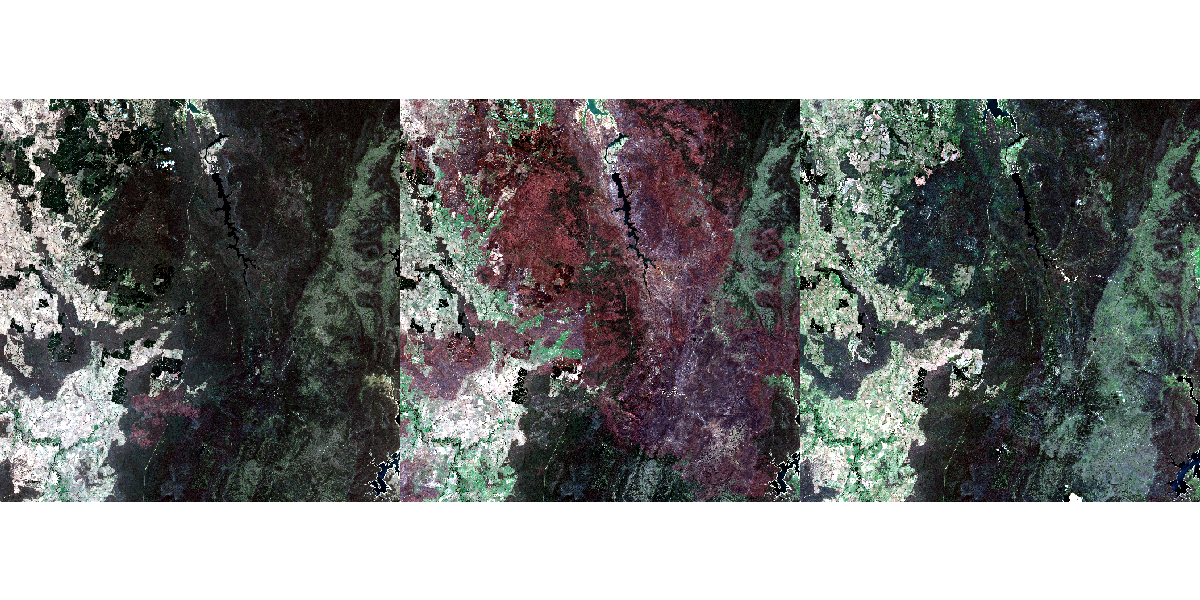
\includegraphics[width=\textwidth]{RGB_comparison.png}
    \caption{RGB 2019-2020-2025}
\end{columns}
\end{frame}

\begin{frame}{\textbf{Immagini RGB in False Color (2019-2020-2025)}}
\begin{columns}
    \column{1\textwidth}
    \centering
    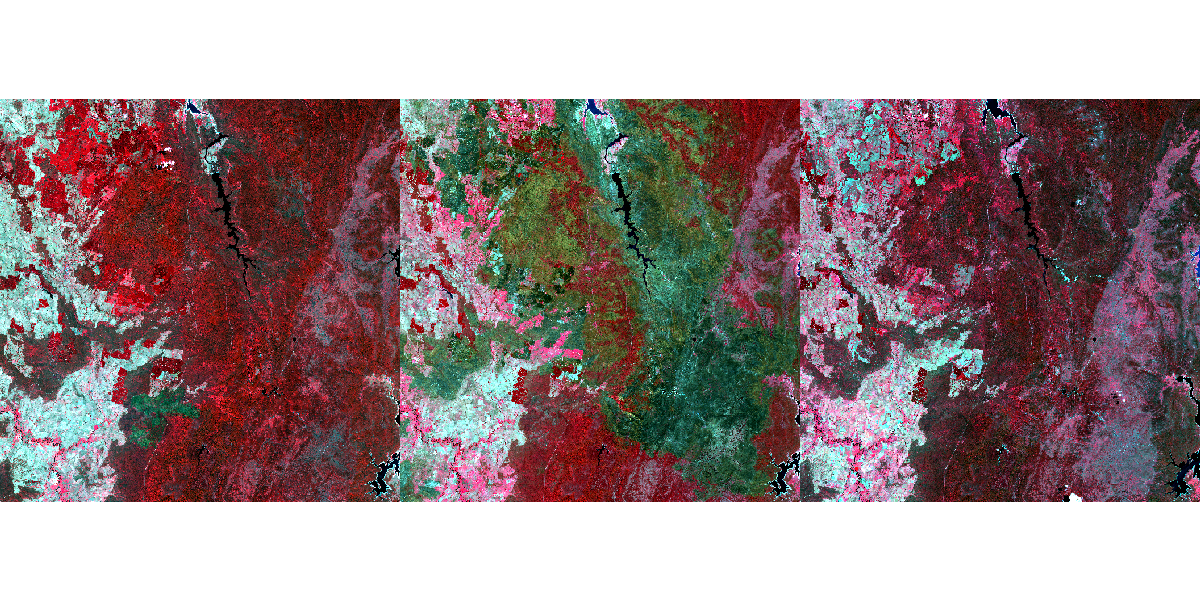
\includegraphics[width=\textwidth]{RGB_comparison_2.png}
    \caption{NIR 2019-2020-2025}
\end{columns}
\end{frame}

\subsection{Software Utilizzati}

\begin{frame}{\textbf{Software Utilizzati}}
\textbf{Software:} R con i seguenti pacchetti:
\begin{itemize}
    \item \texttt{raster}{ per la gestione delle immagini raster}
    \item \texttt{ggplot2}{ per la visualizzazione dei dati}
    \item \texttt{viridis}{ per rappresentare i dati spaziali in modo chiaro ed utile}
\end{itemize}
\end{frame}


\section{Metodologie applicate}

\subsection{Indici Spettrali}

\begin{frame}{\textbf{Indici Spettrali: Definizioni e Formule}}
\textbf{Difference Vegetation Index (DVI):}
\newline
\begin{equation}
\text{DVI} = \text{NIR} - \text{Red}
\end{equation}
\newline
Il DVI misura la densità della vegetazione sottraendo la riflettanza nel rosso dalla riflettanza nell'infrarosso vicino (NIR). 
\newline
Le piante sane riflettono più luce nel NIR rispetto al rosso, quindi un DVI elevato indica una vegetazione densa e sana.
\end{frame}

\begin{frame}[fragile]{\textbf{Calcolo degli Indici Spettrali}}
\textbf{DVI (Difference Vegetation Index):}
\begin{lstlisting}
# Calcolo DVI
DVI_2019 <- img_2019[[4]] - img_2019[[3]] # DVI = NIR - Rosso
#uguale per 2020 e 2025
\end{lstlisting}
\begin{columns}
    \column{1\textwidth}
    \centering
    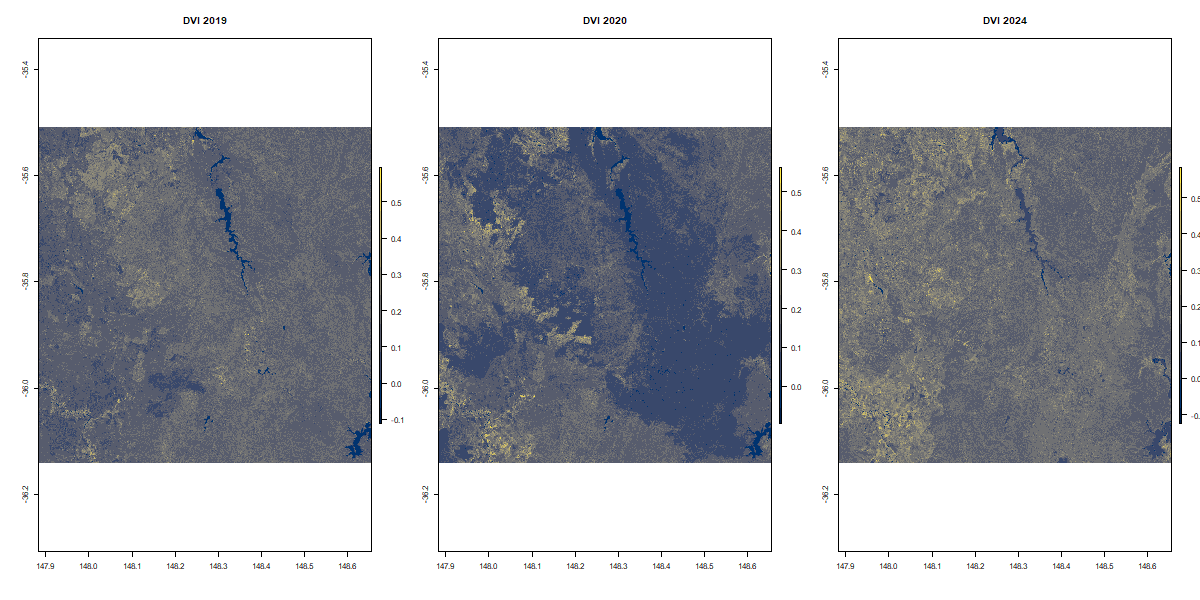
\includegraphics[width=\textwidth]{DVI.png}
\end{columns}
\end{frame}

\begin{frame}{\textbf{Indici Spettrali: Definizioni e Formule}}
\textbf{Normalized Difference Vegetation Index (NDVI):}
\newline
\begin{equation}
\text{NDVI} = \frac{\text{NIR} - \text{Red}}{\text{NIR} + \text{Red}}
\end{equation}
\newline
L'NDVI valuta la salute della vegetazione normalizzando la differenza tra la riflettanza nel NIR e nel rosso.
\end{frame}

\begin{frame}[fragile]{\textbf{Calcolo degli Indici Spettrali}}
\textbf{NDVI (Normalized Difference Vegetation Index):}
\begin{lstlisting}
# Calcolo NDVI
NDVI_2019 <- DVI / (img_2019[[4]] + img_2019[[3]])
# NDVI = DVI/(NIR + Rosso)
#uguale per 2020 e 2025
\end{lstlisting}
\begin{columns}
    \column{1\textwidth}
    \centering
    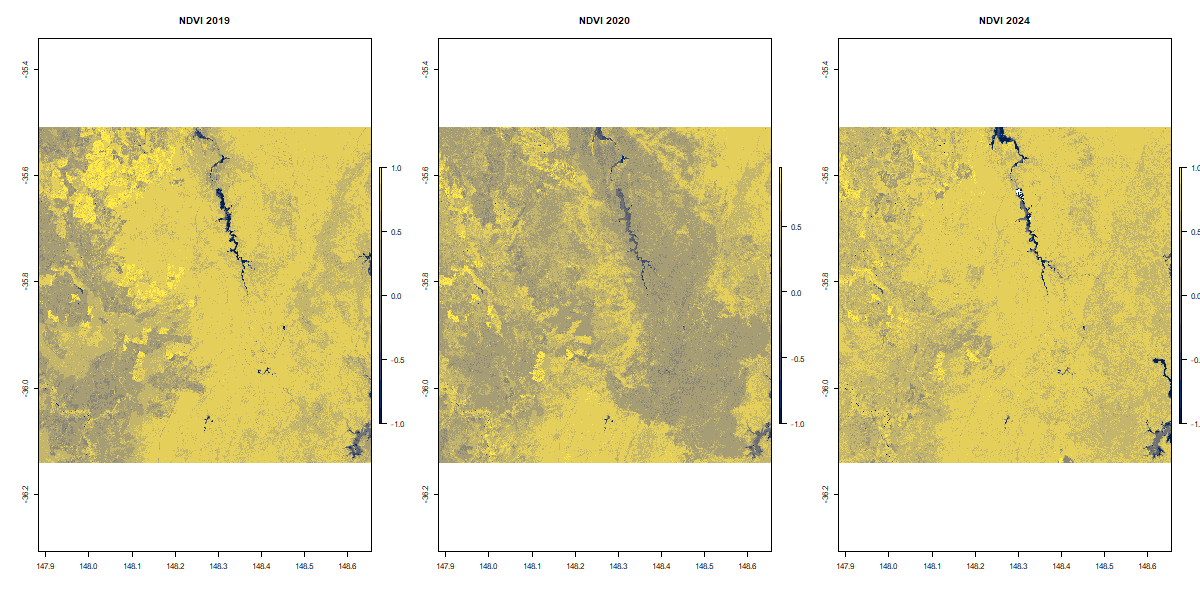
\includegraphics[width=\textwidth]{NDVI.png}
\end{columns}
\end{frame}

\begin{frame}[fragile]{\textbf{Calcolo degli Indici Spettrali}}
\textbf{NDVI (Normalized Difference Vegetation Index):}
\begin{lstlisting}
# Differenze NDVI
NDVI_diff_2020 <- NDVI_2020 - NDVI_2019 
NDVI_diff_2025 <- NDVI_2025 - NDVI_2020 
\end{lstlisting}
\begin{columns}
    \column{1\textwidth}
    \centering
    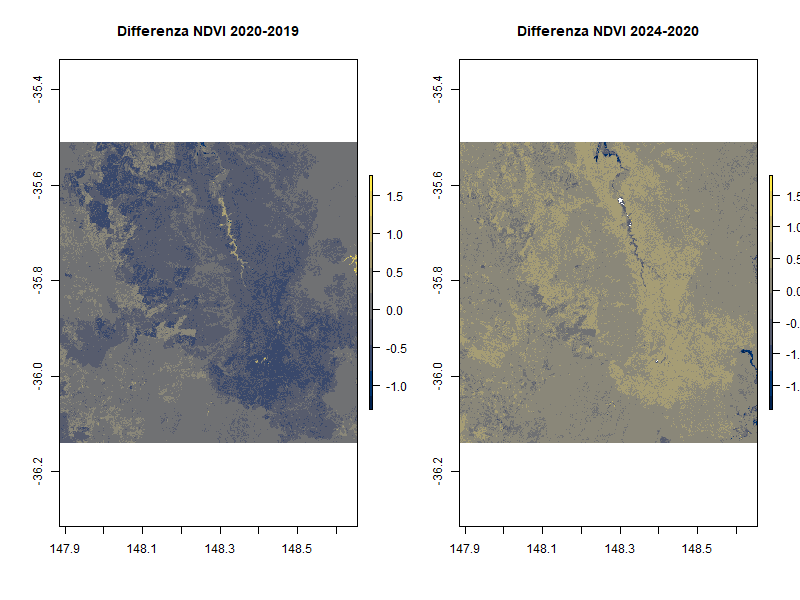
\includegraphics[width=\textwidth]{NDVI_diff.png}
\end{columns}
\end{frame}


\subsection{PCA (Analisi delle Componenti Principali)}

\begin{frame}[fragile]{\textbf{PCA (Analisi delle Componenti Principali)}}
\textbf{Obiettivo:} Ridurre la complessità dei dati di NDVI nei due periodi (2019-2020 e 2020-2025) identificando i principali pattern di cambiamento.

\newline
\newline
\textbf{Procedura:}
\begin{lstlisting}
#PCA sui set di dati (2019-2020 e 2020-2025)
#Creazione dello stack NDVI con la funzione stack
#Campionamento casuale dei pixel con sampleRandom
#Esecuzione della PCA con prcomp
# Proiezione della PCA con la funzione predict
#Infine visualizzazione dei risultati
\end{lstlisting}
\end{frame}

\begin{frame}{\textbf{PCA 2019-2020}}
\begin{columns}
    \column{0.5\textwidth}
    \centering
    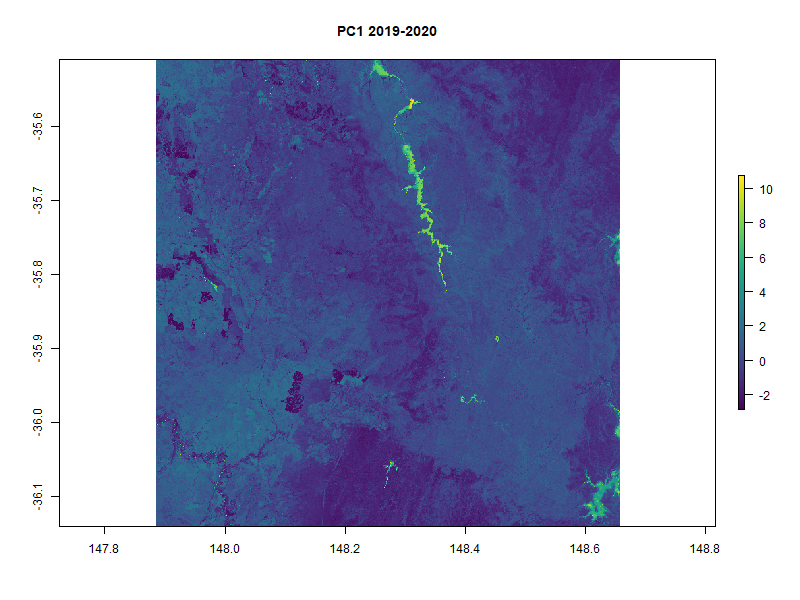
\includegraphics[width=\textwidth]{PCA_PC1_2019_2020.png}
    
    \column{0.5\textwidth}
    \centering
    \textbf{Summary della PCA}
    \begin{table}
        \centering
        \begin{tabular}{lcc}
            \toprule
            & PC1 \\
            \midrule
            Standard deviation     & 1.1246  \\
            Proportion of Variance & 0.6324 \\
            \bottomrule
        \end{tabular}
    \end{table}
\end{columns}
\end{frame}

\begin{frame}{\textbf{PCA 2020-2025}}
\begin{columns}
    \column{0.5\textwidth}
    \centering
    \includegraphics[width=\textwidth]{PCA_PC1_2020_2025.png}
    
    \column{0.5\textwidth}
    \centering
    \textbf{Summary della PCA}
    \begin{table}
        \centering
        \begin{tabular}{lcc}
            \toprule
            & PC1 \\
            \midrule
            Standard deviation     & 1.123 \\
            Proportion of Variance & 0.630 \\
            \bottomrule
        \end{tabular}
    \end{table}
\end{columns}
\end{frame}


\subsection{Classificazione Land Cover}

\begin{frame}[fragile]{\textbf{Classificazione Land Cover}}
\textbf{Obiettivo:} Classificare l'area di studio in due categorie di copertura vegetale ("buona", "ridotta/assente") utilizzando l'algoritmo di clustering K-Means. Per osservare e quantificare meglio i cambiamenti nella copertura vegetale nel tempo.
\newline
\newline
\textbf{Procedura:}
\begin{lstlisting}
#Classificazione Land Cover nei diversi anni (2019, 2020 e 2025)
#imposto il seme per la riproducibilità con set.seed(2)
#Estraggo i valori dei pixel con getValues()
#clusterizzo con kmeans() indicando il numero di centri
#Creo l'immagine classifica tramite setValues()
#Calcolo delle frequenze con freq() e ncell()
\end{lstlisting}
\end{frame}

\begin{frame}{\textbf{Immagini Classificazione Land Cover}}
\begin{columns}
    \column{0.33\textwidth}
    \centering
    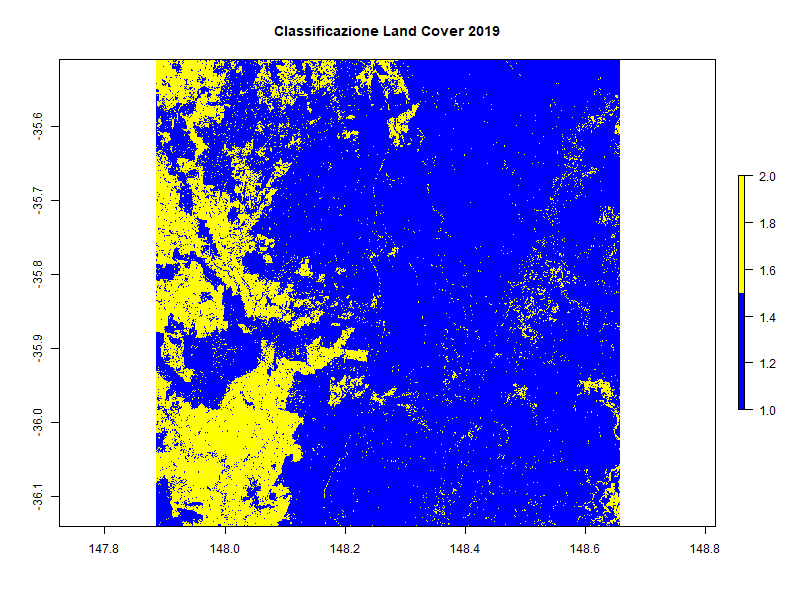
\includegraphics[width=\textwidth]{Land_Cover_2019.png}
    \caption{Land Cover 2019}

    \column{0.33\textwidth}
    \centering
    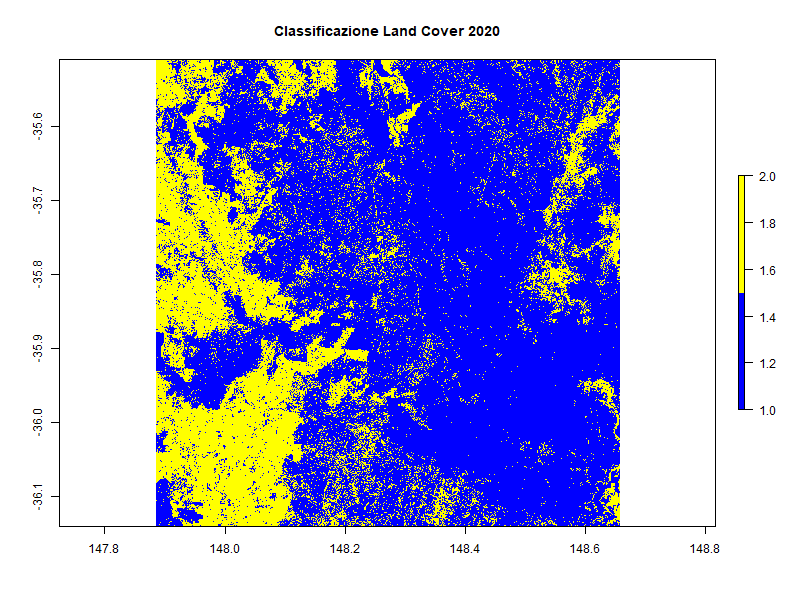
\includegraphics[width=\textwidth]{Land_Cover_2020.png}
    \caption{Land Cover 2020}

    \column{0.33\textwidth}
    \centering
    \includegraphics[width=\textwidth]{Land_Cover_2025.png}
    \caption{Land Cover 2025}
\end{columns}
\end{frame}

\begin{frame}{\textbf{Percentuali di Copertura Vegetale}}
\begin{columns}
    \column{0.33\textwidth}
    \centering
    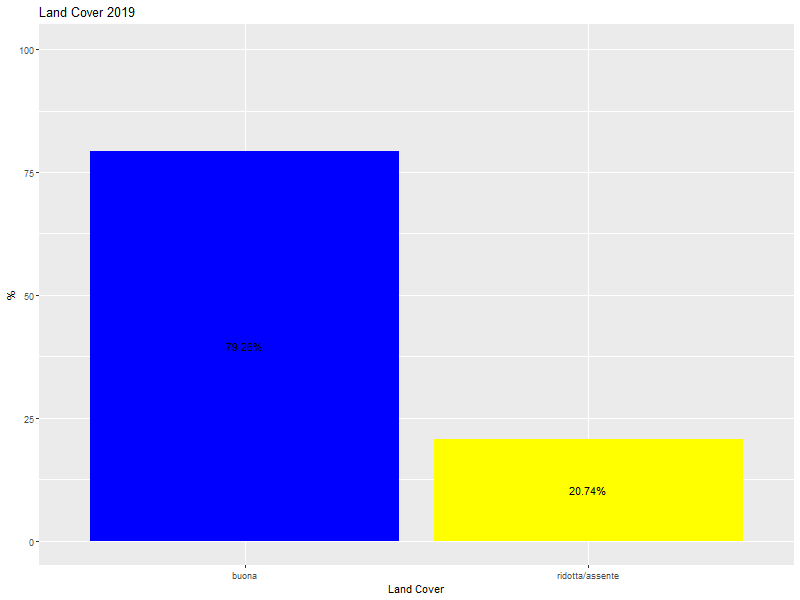
\includegraphics[width=\textwidth]{Percentuali_Land_Cover_2019.png}
    \caption{Percentuali Land Cover 2019}

    \column{0.33\textwidth}
    \centering
    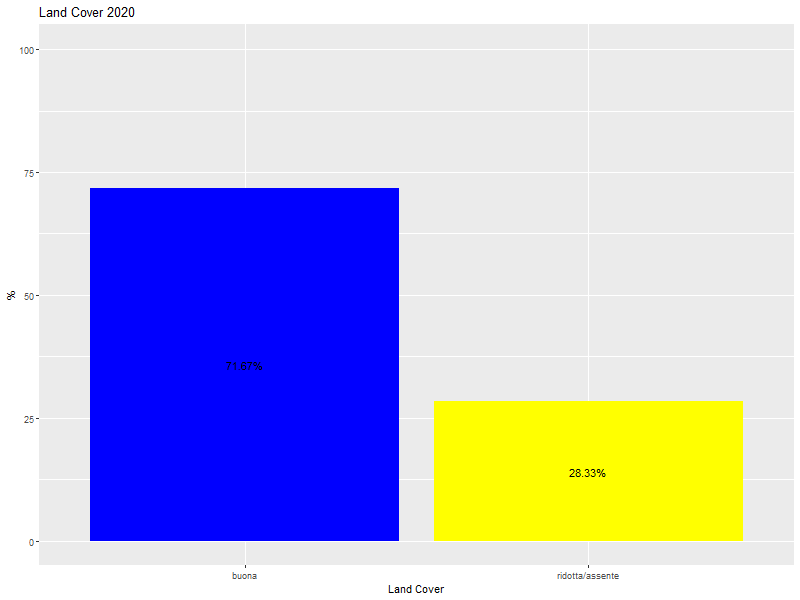
\includegraphics[width=\textwidth]{Percentuali_Land_Cover_2020.png}
    \caption{Percentuali Land Cover 2020}

    \column{0.33\textwidth}
    \centering
    \includegraphics[width=\textwidth]{Percentuali_Land_Cover_2025.png}
    \caption{Percentuali Land Cover 2025}
\end{columns}
\end{frame}

\subsection{T-Test}
\begin{frame}[fragile]{\textbf{T-Test}}
\textbf{Obiettivo:} Determinare se c'è una differenza significativa tra i valori medi di NDVI (Normalized Difference Vegetation Index) nei due anni confrontati.
\newline
\newline
\textbf{Procedura:}
\begin{lstlisting}
# Estrazione dei valori NDVI dai raster dei tramite getValues
# T-test tra i due set di dati con t.test()
# Stampo i risultati con print()
\end{lstlisting}
\end{frame}

\begin{frame}[fragile]{\textbf{T-Test}}
\textbf{Risultati T-Test:}
\begin{itemize}
    \item \textbf{T-test tra 2019 e 2020:}
    \begin{itemize}
        \item t = 3696.3, df = 11503862, p-value < 2.2e-16
        \item 95 percent confidence interval: 0.3565054 - 0.3568836
        \item mean of x = 0.6730575, mean of y = 0.3163630
        \newline
        \item La media di NDVI è diminuita significativamente (p-value < 2.2e-16) dal 2019 al 2020, con una riduzione media di circa 0.356 che indica una perdita di copertura vegetale.
    \end{itemize}
\end{itemize}
\end{frame}

\begin{frame}[fragile]{\textbf{T-Test}}
\textbf{Risultati T-Test 2020-2025:}
\begin{itemize}
     \item \textbf{T-test tra 2020 e 2025:}
    \begin{itemize}
        \item t = -3679.7, df = 11438646, p-value < 2.2e-16
        \item 95 percent confidence interval: -0.3334739 - -0.3331188
        \item mean of x = 0.3163630, mean of y = 0.6496593
        \newline
        \item NDVI è aumentato significativamente tra il 2020 e il 2025. La differenza media è di circa -0.333, con un'elevata significatività statistica (p-value < 2.2e-16).
    \end{itemize}
\end{itemize}
\end{frame}


\section{Conclusioni}
\begin{frame}[fragile]{\textbf{Conclusioni}}
\textbf{Impatto degli incendi:} Gli incendi del 2019 hanno provocato una drastica riduzione della copertura vegetale, come evidenziato dai valori di NDVI e DVI nel confronto tra il 2019 e il 2020 sia tramite PCA che Land Cover. Il t-test conferma che questa riduzione è statisticamente significativa (p-value < 2.2e-16).
\end{frame}

\begin{frame}[fragile]{\textbf{Conclusioni}}
\textbf{Ripresa della vegetazione:} Dal 2020 al 2025 si osserva una graduale ripresa della vegetazione, con un aumento significativo dei valori medi di NDVI (incremento medio di 0.333), testimoniando un progressivo ritorno della salute ecologica dell'area.
\end{frame}

\begin{frame}[fragile]{\textbf{Conclusioni}}
\textbf{Pattern spaziali:} L’analisi delle componenti principali (PCA) ha permesso di individuare le aree con maggiore vulnerabilità, suggerendo che alcune aree del parco abbiano mostrato una resilienza maggiore rispetto ad altre.
\end{frame}

\section{Prospettive future}
\begin{frame}[fragile]{\textbf{Prospettive future}}
\textbf Sarebbe interessante ampliare l'analisi statistica del progetto, includendo un maggior numero di anni per verificare l'andamento del ripristino della vegetazione. 
Inoltre, sarebbe utile continuare il monitoraggio anche negli anni futuri.  
\end{frame}

\begin{frame}{}
\centering
\textbf{Grazie per l'attenzione!}
\end{frame}

\end{document}
